\chapter{Design}
This chapter describes how the PCB has been designed in order to obtain EMC. The different laws used and reviews with supervisor \textit{Per Lysgaard} are also described. 

%\todo[inline]{Description of how you expect your design can comply with existing laws (how the system and PCB has been designed to obtain EMC).\\ Short description of which laws the system must comply to.\\ Description of reviews we've had with Per.}
\section{Standards}
The different European standards according to Electromagnetic compatibility is found on the European Commission website \footnote{\url{http://ec.europa.eu/enterprise/policies/european-standards/harmonised-standards/electromagnetic-compatibility/index\_en.htm\#Note 2.3}}.
The standard: \textit{EN 50412-2-1:2005} deals with: \textit{Power line communication apparatus and systems used in low-voltage installations in the frequency range 1.6 MHz to 30 MHz}. However, the power line is not to work on a low-voltage installation but in an isolated DC environment. Another reason why not to use this standard is its expire date: 01/04/2008. Instead of this standard a generic standard is used.

\begin{figure}[H]
	\begin{centering}
		 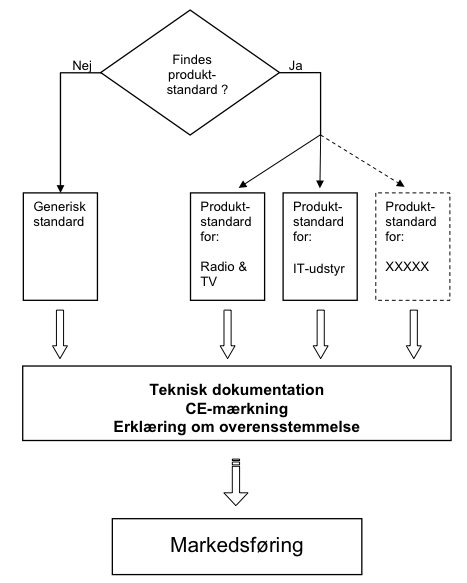
\includegraphics[width=0.5\textwidth]{images/choose_hormonic_standard.png}
		\caption{Choosing a relevant generic standard.}
	\end{centering}
\end{figure}
Basically there are two different generic standards both when talking immunity and emission. The standards are either residential or industrial. The definition of an industry is a place with its own transformer station. As the power line module can be used both places a mix is chosen, where the immunity test have to withstand the demands for industrial implementation and the emission have to withstand the demands for residential implementation. In the industry there is a high requirement of immunity on the devices and low requirement for emission. This is vice versa for the residential requirements. The standards used is therefore:
	\begin{itemize}
		\item \textit{61000-6-2} for immunity (industrial requirements)
		\item \textit{61000-6-3} for emission (residential requirements)
	\end{itemize}
The two standards describes what demands the equipment have to fulfill, how the tests should be done and how the measurements should be reported. 
\subsection{Schematic and first PCB layout}
Full documentation of the schematic design can be found in the Appendix \textit{EPRO\_3\_\&\_4\_PLC - Hardware}. The design consists of two parts, a SMPS (switch mode power supply) and a PLC (power line communication) module. Both modules takes input from the power line (30VDC), where the Power Line part filters out the communication on top of the DC voltage and also sends commands to other modules on the net. The SMPS converts the 30VDC input to a 5VDC supply that can be used to power the Processor board and the FPGA board used in the project\footnote{EPRO4}. The PCB has been divided into two sections with the 30VDC connection in between the two modules to have as little interference as possible.
\begin{figure}[H]
	\begin{centering}
		 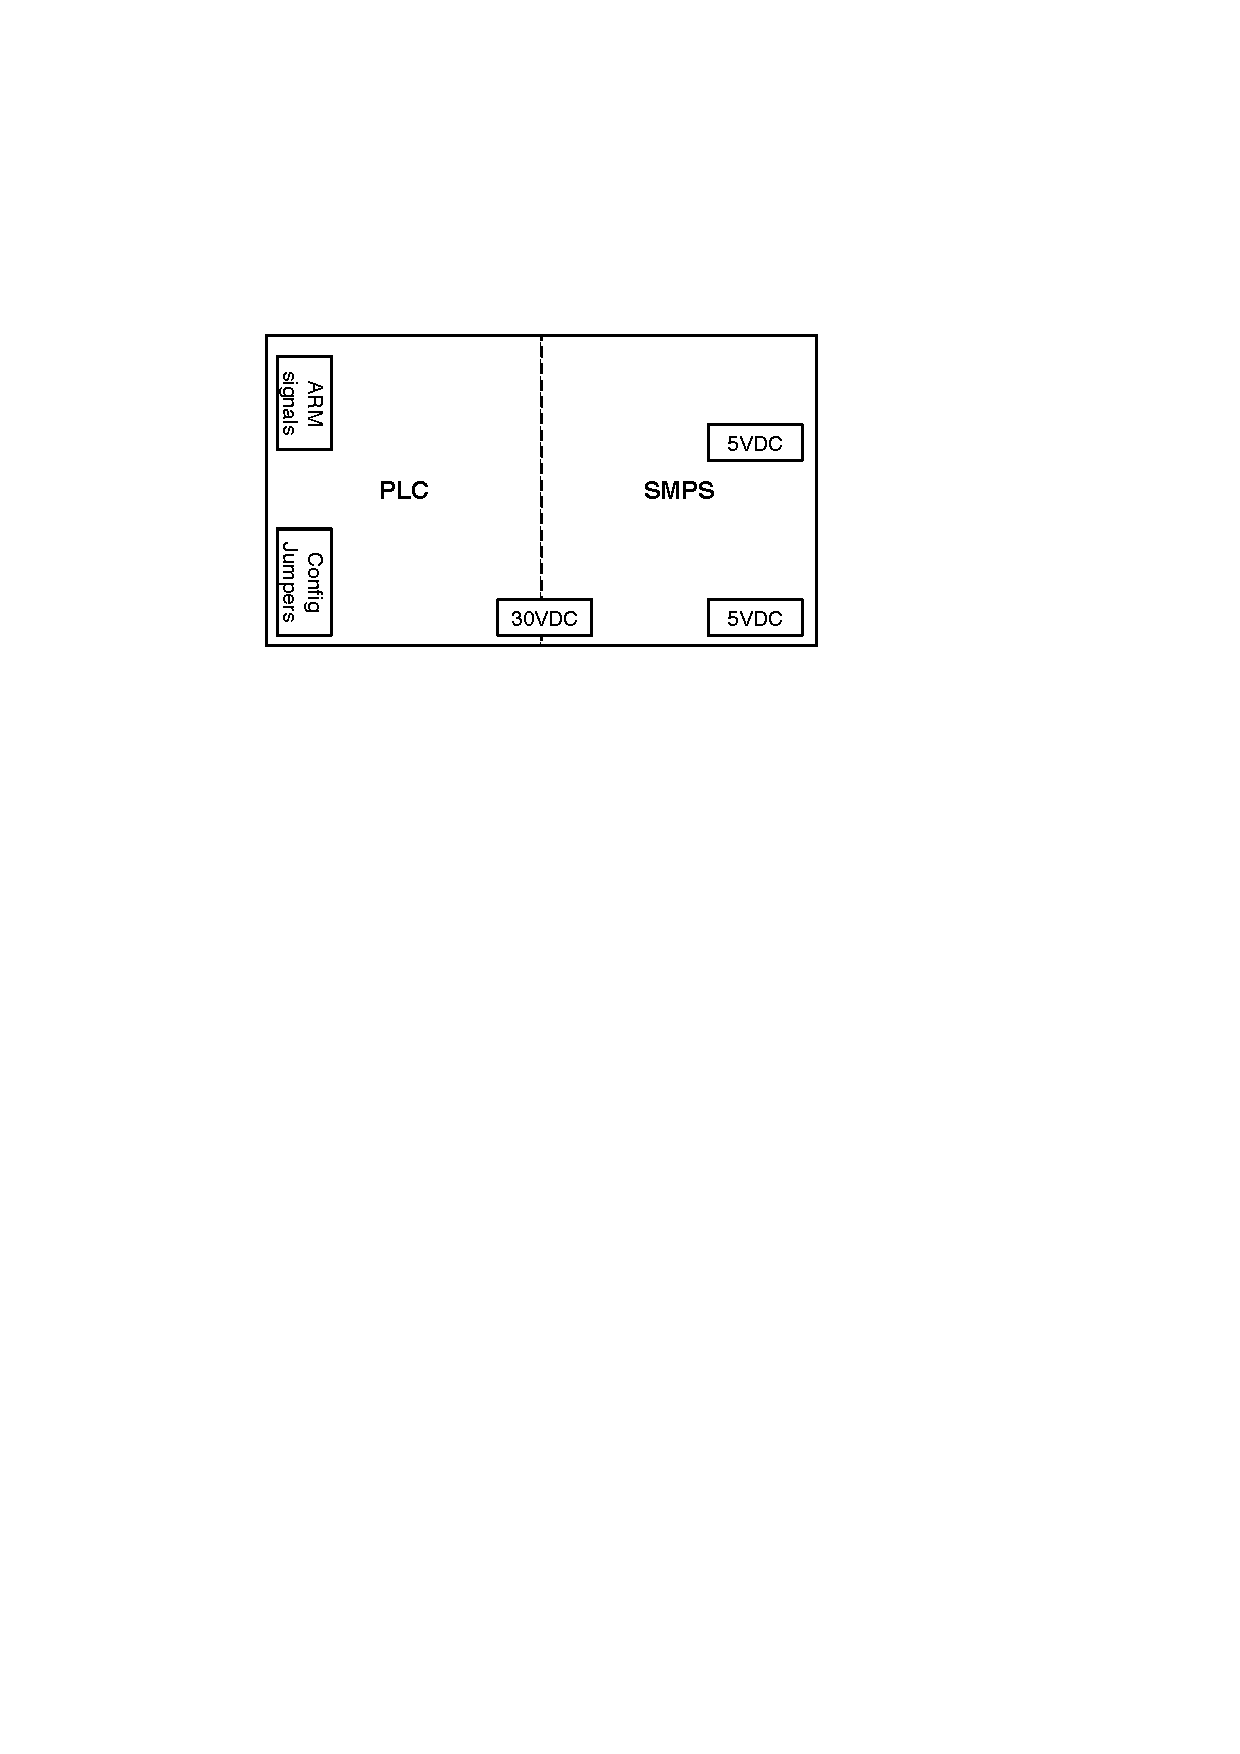
\includegraphics[width=0.5\textwidth]{images/pcb_design.pdf}
		\caption{Overview of how the board is divided (Setup of the final board).}
		\label{fig:board_overview}
	\end{centering}
\end{figure}

\subsubsection{Schematic}
The schematic has only changed slightly during the different versions of the circuit board. Down below the newest version of the schematic is shown (the PCB that fits to the schematic is shown in review 2).
\begin{figure}[H]
	\begin{centering}
		 \includegraphics[width=0.85\textwidth,page=2,angle=0]{images/SIG60_v0_4}
		\caption{Communication part of the design.}
	\end{centering}
\end{figure}

\begin{figure}[H]
	\begin{centering}
		 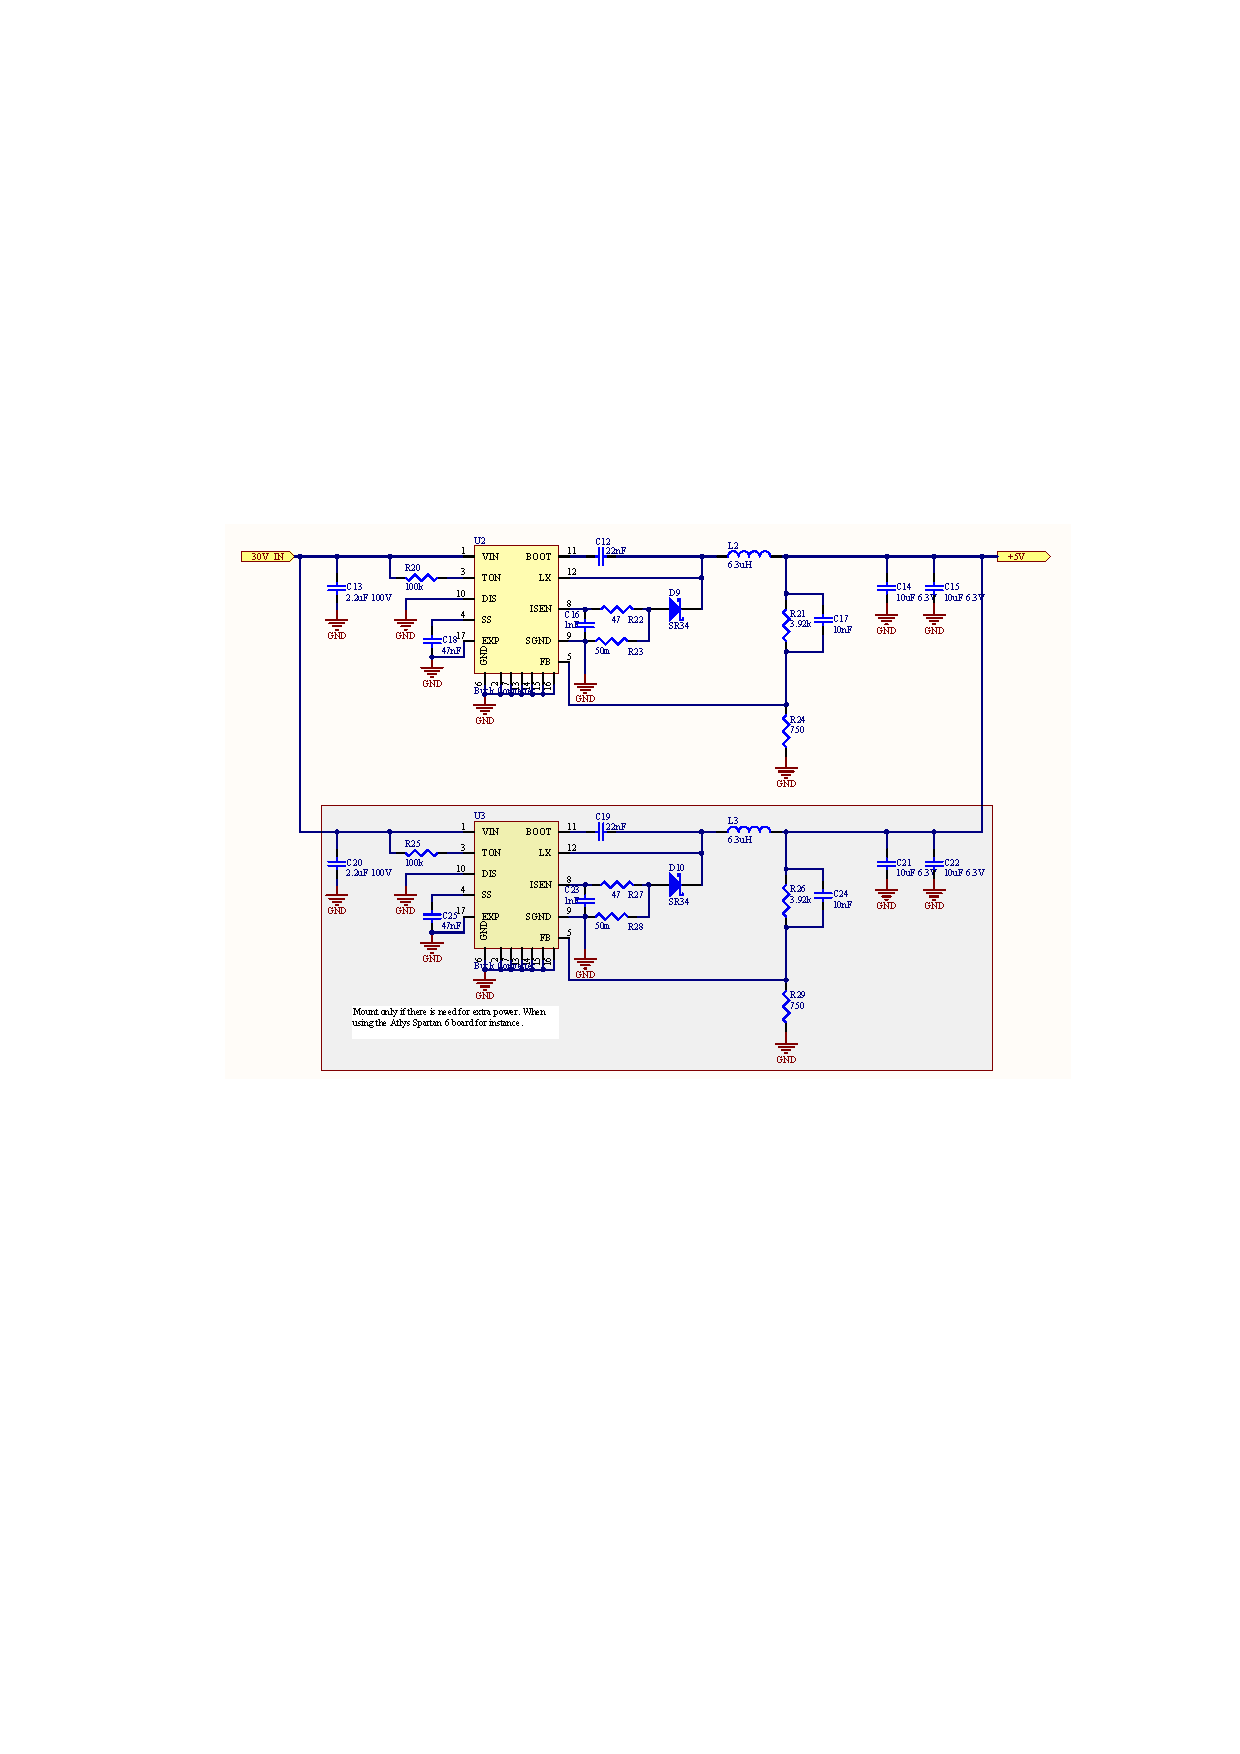
\includegraphics[width=0.85\textwidth,page=1,angle=0]{images/SIG60_v0_4}
		\caption{Power supply section of the design.}
	\end{centering}
\end{figure}

\subsection{Review 1}
The first PCB layout was made before attending the EMC course in the start of February 2012. In the end of the course feedback for the design was given. Basically two things should be changed:
\begin{itemize}
	\item Shorten tracks on bottom side, so a clean ground plane is held. 
	\item Enlarge track width (especially power tracks).
\end{itemize}

\begin{figure}[H]
	\begin{centering}
		 \includegraphics[width=0.6\textwidth,page=3,angle=0]{images/SIG60_v0_1}
		\caption{First routing of the circuit-board.}
	\end{centering}
\end{figure}

\subsection{Review 2}
In the second layout all track widths were adjusted, track length shortened and the amount of long tracks on the ground plane minimized. The only remark for this design was one of the tracks on the ground plane at twice the length of the other tracks. A PCB was made with this design as the remark was not critical and a redesign would require quiet some time.
\\\textit{Note: the free space on the PCB was connected to ground on both planes.}
\begin{figure}[H]
	\begin{centering}
		 \includegraphics[width=0.6\textwidth,page=3,angle=0]{images/SIG60_v0_2}
		\caption{First redesign of the PCB layout.}
	\end{centering}
\end{figure}
\subsubsection{Testing the PCB}
Testing of the first PCB is documented in the Appendix \textit{EPRO\_3\_\&\_4\_PLC - Hardware}. A short resume:
\begin{itemize}
	\item The output of the switch mode was unstable when loaded. 
	\begin{itemize}
		\item The feedback track shall be made shorter and the width of it enlarged. 
		\item Generally all components shall be placed closer to the switch mode device to shorten track lengths. 
		\item More vias for better connection to the ground plane, if it is possible, one or more should be placed underneath the switch mode device.
	\end{itemize}
	\item When noise was added to the power line, random characters appeared in the communication.
	\begin{itemize}
		\item A big resister has been added between the receive pin and ground.
		\item Filters and crystal shall be placed as close as possible to the power line device to decrease the noise furthermore.
	\end{itemize} 
	\item The receive diode lightens up all the time.
	\begin{itemize}
		\item The diode shall use the RxOn pin on the Power Line device instead of the receive pin to fix the problem.
	\end{itemize}
\end{itemize}

\subsection{Final design}
%Reroute filters + Switch mode feedback.
In the final layout, all components have been placed even closer to the different IC's. The board size has decreased to approximately 65\% of the last version. 
\\ To ease mounting, all vias and pads have been increased in size. As the pin-headers shall be soldered on both sides, the pads have also been shaped oblongly. Clearance between the tracks is defined to 15 mil as this distance can easily be made on homemade PCB's. 
\\ The 5 volt output tracks should be able to withstand 3 amperes maximum, according to the book \textit{PCB Design Tutorial page 7} (see appendix), the track size shall be minimum 50mil. A width of 60 mil have been chosen. 
\\ As it can be seen on fig: \ref{fig:board_overview} how the connectors on the board is placed. Usually it is preferable to have all connections in one side of a PCB (possible two). Although, to keep tracks as short as possible, and to place the shared item (30 Volt plug) a central place for both sides of the PCB, this rule has not been kept strict.
%increased pad size
%Placement of 30 volt plug

% connections in the side of the PCB (except 30 volt)
% Power Track size 60mil, 50mil to withstand 3Amp 


\begin{figure}[H]
	\begin{centering}
		 \includegraphics[width=0.55\textwidth,page=3,angle=0]{images/SIG60_v0_4}
		\caption{Final version of the PCB.}
	\end{centering}
\end{figure}


\begin{figure}[H]
	\begin{centering}
		 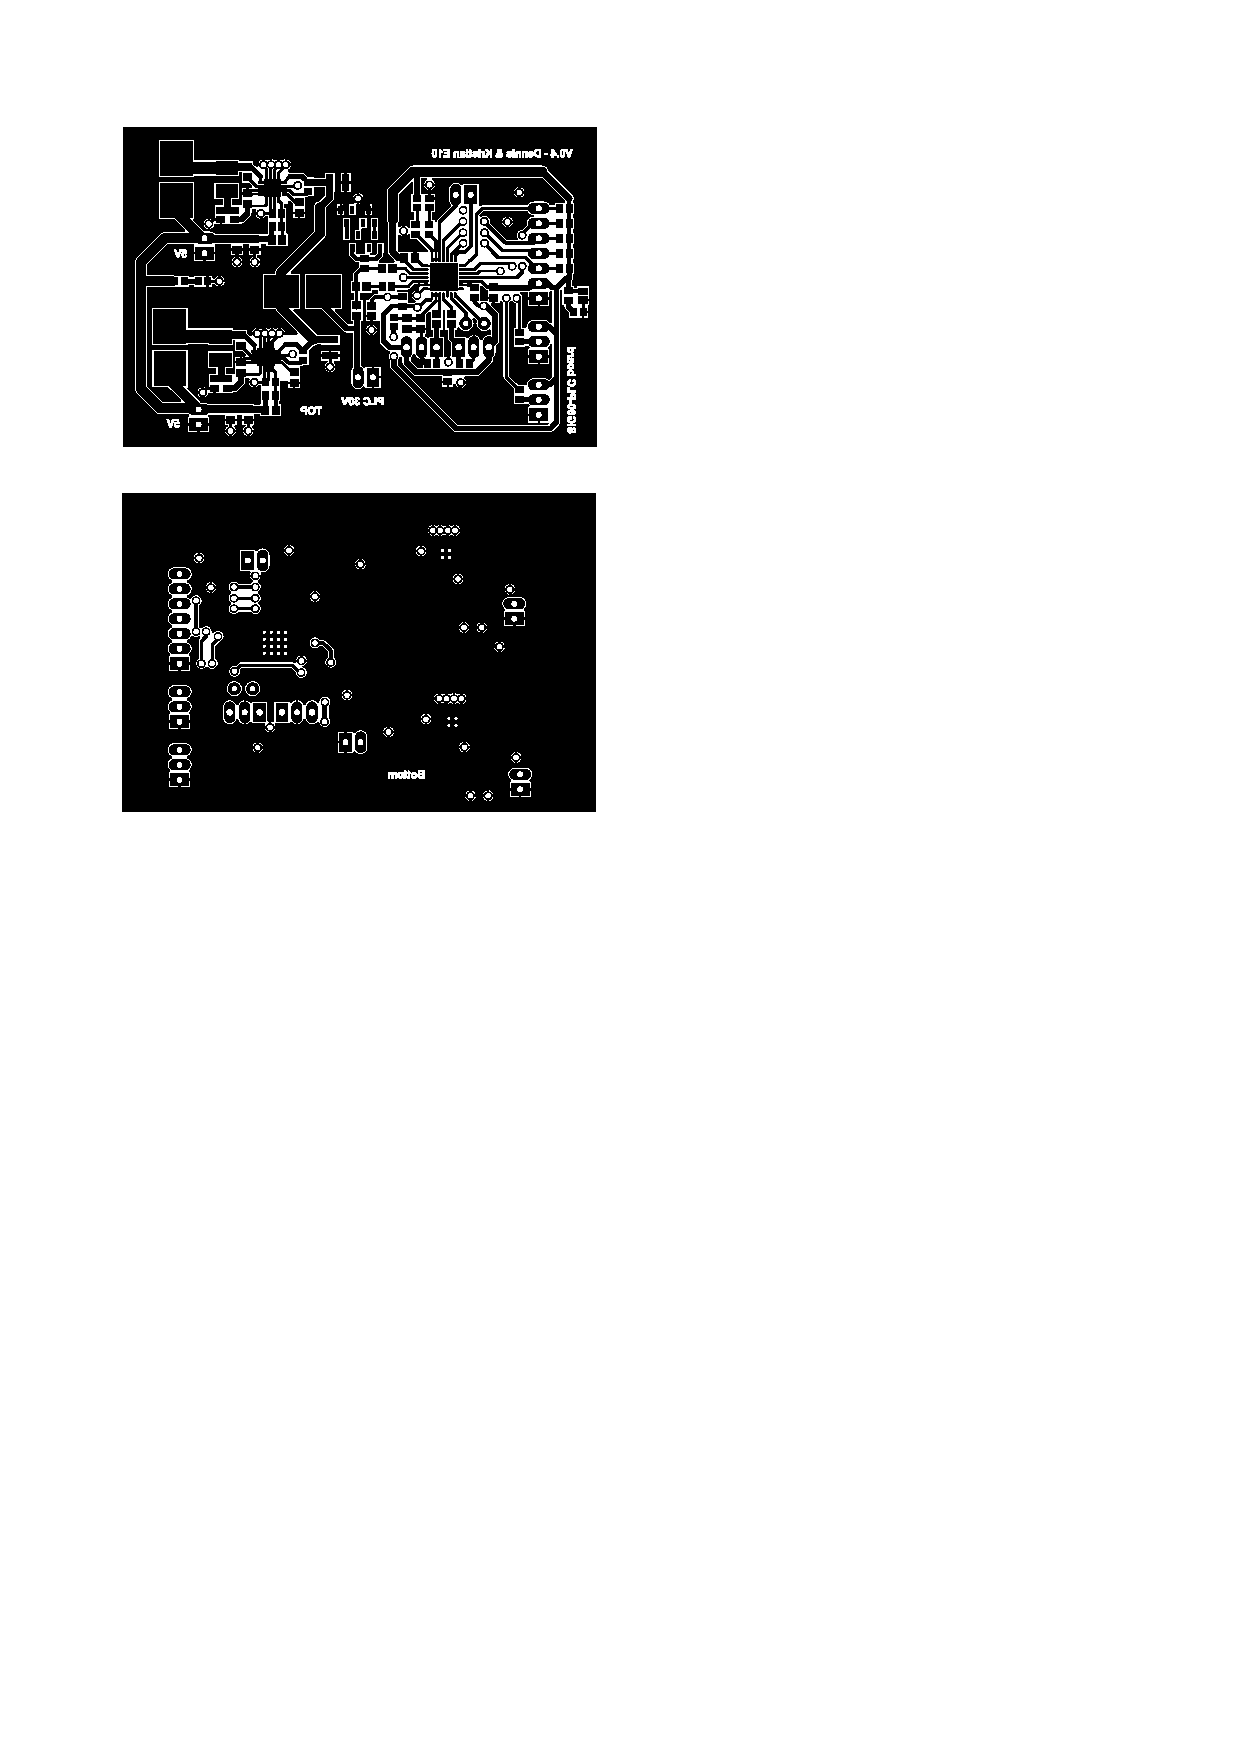
\includegraphics[page=1,angle=90]{images/jens_print_4}
		\caption{PCB layout, top and bottom}
	\end{centering}
\end{figure}

\begin{figure}[H]
	\begin{centering}
		 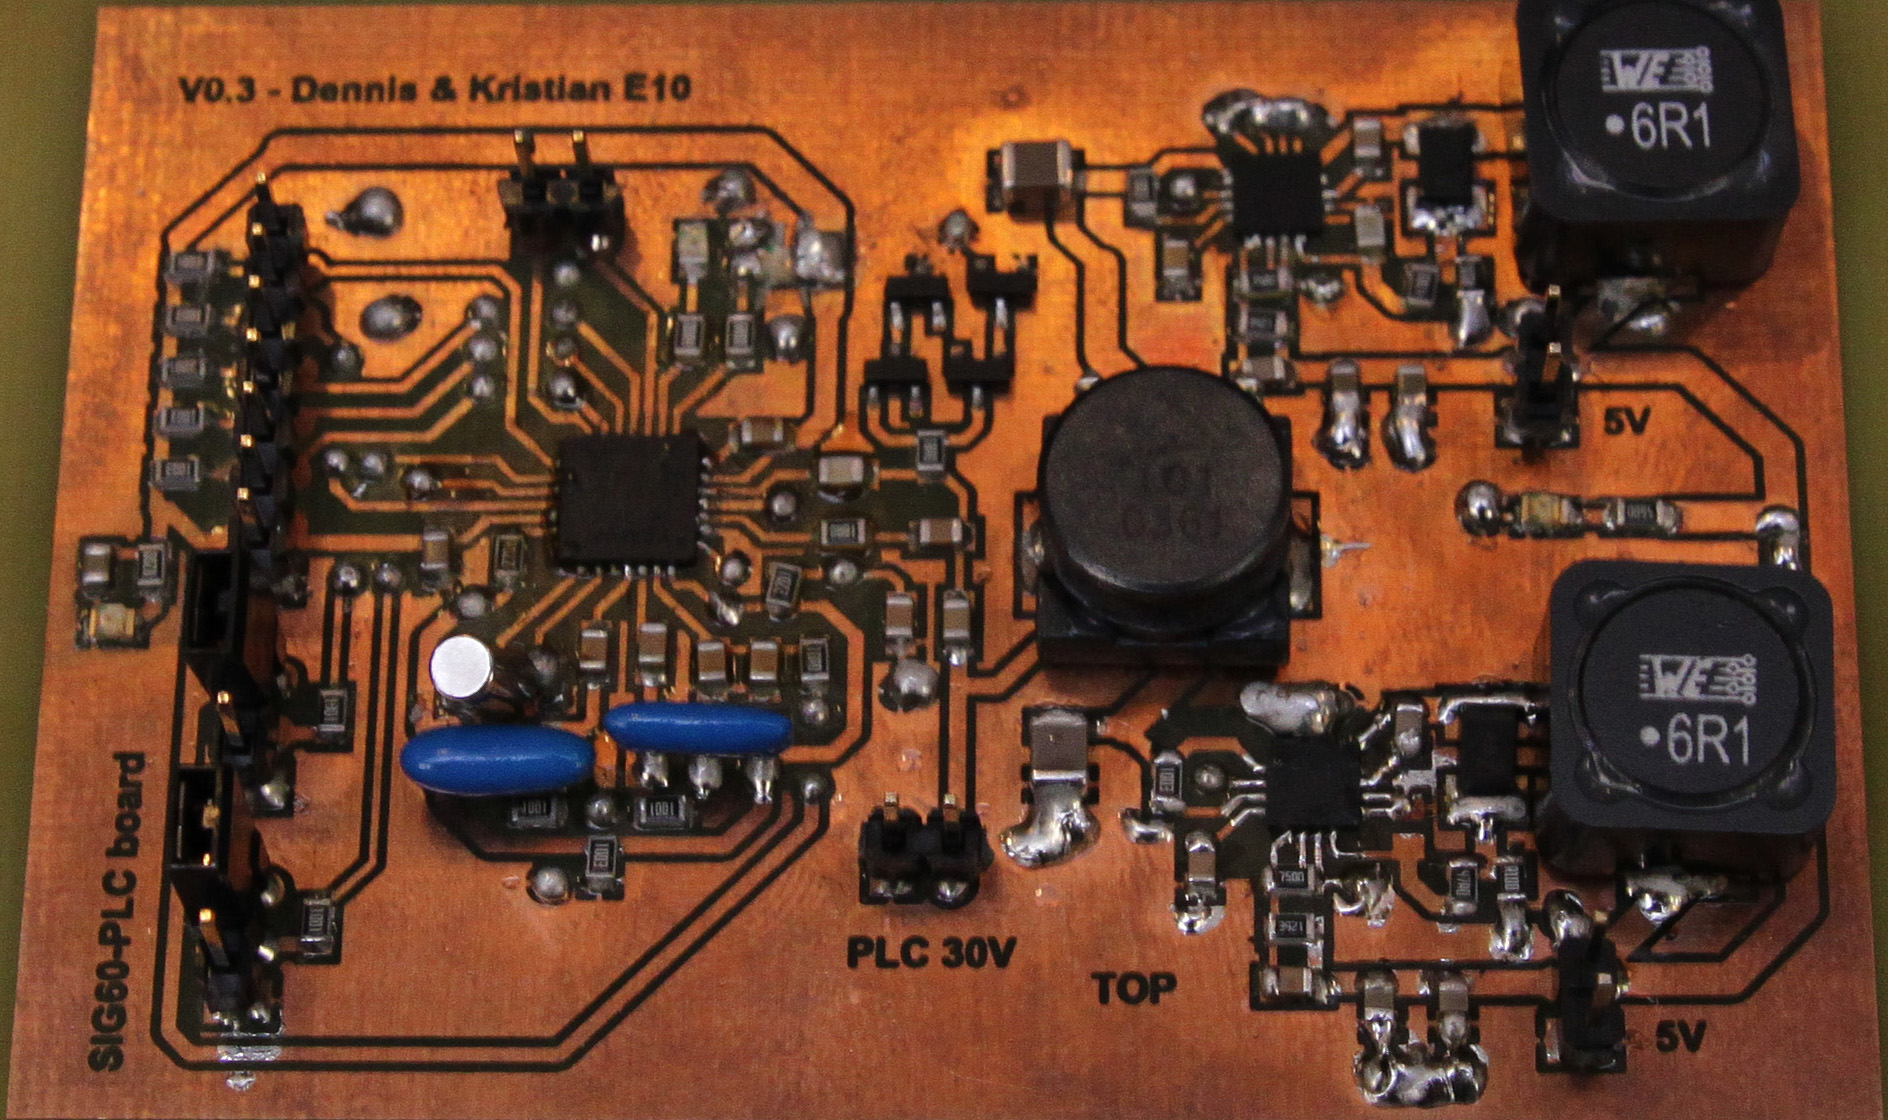
\includegraphics[width=0.8\textwidth]{images/final_board.jpg}
		\caption{Final PCB mounted with both switch mode supplies}
	\end{centering}
\end{figure}
